\ifnum \Version=6
\question[3] Consider the system $$\vec x \, ' = A\vec x, \quad A = \begin{pmatrix} -3&-4\\1&-1 \end{pmatrix}, \quad \vec x = \begin{pmatrix} x(t)\\y(t)\end{pmatrix} $$ The eigenvalues of $A$ are $\lambda = -2\pm i\sqrt 3$. Sketch the phase portrait of the system. Sketch at least two solution curves. Please indicate the direction of motion on your solution curves. Don't forget to label your axes.   

\ifnum \Solutions=1 {\color{DarkBlue} 
\textbf{Solutions:} solution curves should \textbf{spiral towards} the origin and rotate \textbf{counter clockwise}. Axes should be labelled. Ok to only draw only two solution curves. 
    \begin{center}
    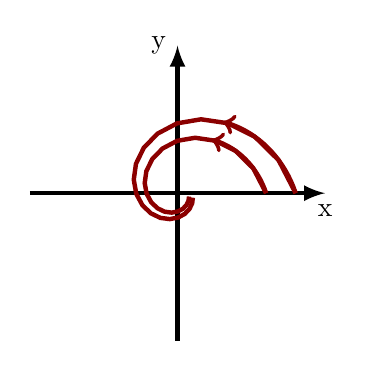
\begin{tikzpicture}[scale=0.75]
      \draw[ultra thick,->,>=latex] (-2.5,0)--(2.5,0) node[below] {x};
      \draw[ultra thick,->,>=latex] (0,-2.5)--(0,2.5) node[left] {y};      
      \draw[domain=0:6,ultra thick,samples=20,DarkRed] plot ({cos(deg(\x))*2*exp(-\x/3},{sin(deg(\x))*2*exp(-\x/3});
      \draw[domain=0:1,->,ultra thick,samples=20,DarkRed] plot ({cos(deg(\x))*2*exp(-\x/3},{sin(deg(\x))*2*exp(-\x/3});
      \draw[domain=0:6,ultra thick,samples=20,DarkRed] plot ({.75*cos(deg(\x))*2*exp(-\x/3},{.75*sin(deg(\x))*2*exp(-\x/3});
      \draw[domain=0:1,->,ultra thick,samples=20,DarkRed] plot ({.75*cos(deg(\x))*2*exp(-\x/3},{.75*sin(deg(\x))*2*exp(-\x/3});
    \end{tikzpicture}
    \end{center} 
} 
\else 
    \begin{center}
    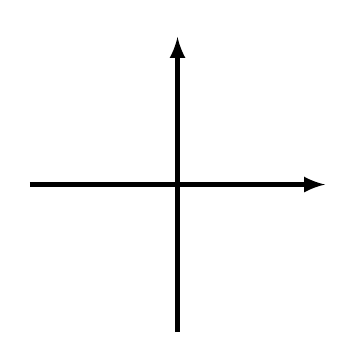
\begin{tikzpicture}[scale=0.75]
      \draw[ultra thick,->,>=latex] (-2.5,0)--(2.5,0) node[below] {};
      \draw[ultra thick,->,>=latex] (0,-2.5)--(0,2.5) node[left] {};         
    \end{tikzpicture}
    \end{center} 
\fi
\fi


\ifnum \Version=7
\question[3] Consider the system $$\vec x \, ' = A\vec x, \quad A = \begin{pmatrix} 3&2\\-5&1 \end{pmatrix}, \quad \vec x = \begin{pmatrix} x(t)\\y(t)\end{pmatrix} $$ The eigenvalues of $A$ are $\lambda = 2\pm  3i$. Sketch the phase portrait of the system. Sketch at least two solution curves. Please indicate the direction of motion on your solution curves. Don't forget to label your axes.   

\ifnum \Solutions=1 {\color{DarkBlue} 
\textbf{Solutions:} solution curves should \textbf{spiral away} from the origin and rotate \textbf{clockwise}. Axes should be labelled. Ok to only draw only two solution curves. 
\begin{center}
    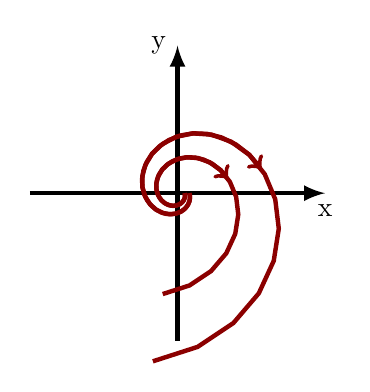
\begin{tikzpicture}[scale=0.75]
      \draw[ultra thick,->,>=latex] (-2.5,0)--(2.5,0) node[below] {x};
      \draw[ultra thick,->,>=latex] (0,-2.5)--(0,2.5) node[left] {y};      
      \draw[domain=0:8,ultra thick,samples=30,DarkRed] plot ({cos(deg(\x))*0.12*exp(\x/3)},{-sin(deg(\x))*0.12*exp(\x/3)});
      \draw[domain=0:6,->,ultra thick,samples=30,DarkRed] plot ({cos(deg(\x))*0.12*exp(\x/3)},{-sin(deg(\x))*0.12*exp(\x/3)});
      \draw[domain=0:8,ultra thick,samples=30,DarkRed] plot ({cos(deg(\x))*0.2*exp(\x/3)},{-sin(deg(\x))*0.2*exp(\x/3)});
      \draw[domain=0:6,->,ultra thick,samples=30,DarkRed] plot ({cos(deg(\x))*0.2*exp(\x/3)},{-sin(deg(\x))*0.2*exp(\x/3)});      
    \end{tikzpicture}
\end{center} 
} 
\else 
\begin{center}
    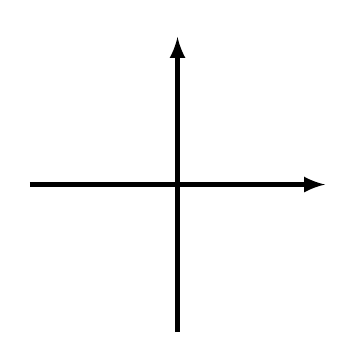
\begin{tikzpicture}[scale=0.75]
      \draw[ultra thick,->,>=latex] (-2.5,0)--(2.5,0) node[below] {};
      \draw[ultra thick,->,>=latex] (0,-2.5)--(0,2.5) node[left] {};         
    \end{tikzpicture}
\end{center} 
\fi
\fi






\ifnum \Version=8
\question[3] Consider the system $$\vec x \, ' = A\vec x, \quad A = \begin{pmatrix} -3&-4\\1&-1 \end{pmatrix}, \quad \vec x = \begin{pmatrix} x(t)\\y(t)\end{pmatrix} $$ The eigenvalues of $A$ are $\lambda = -2\pm i\sqrt 3$. Sketch the phase portrait of the system. Sketch at least two solution curves. Please indicate the direction of motion on your solution curves. Don't forget to label your axes.   

\ifnum \Solutions=1 {\color{DarkBlue} 
\textbf{Solutions:} solution curves should spiral towards center and rotate counter clockwise. Axes should be labelled. Ok to only draw only two solution curves. 
    \begin{center}
    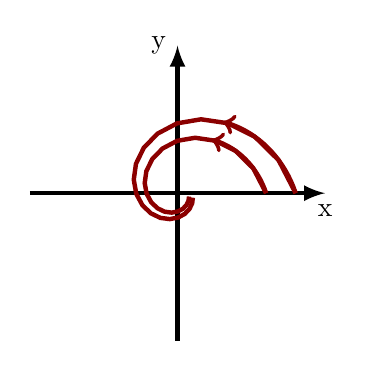
\begin{tikzpicture}[scale=0.75]
      \draw[ultra thick,->,>=latex] (-2.5,0)--(2.5,0) node[below] {x};
      \draw[ultra thick,->,>=latex] (0,-2.5)--(0,2.5) node[left] {y};      
      \draw[domain=0:6,ultra thick,samples=20,DarkRed] plot ({cos(deg(\x))*2*exp(-\x/3},{sin(deg(\x))*2*exp(-\x/3});
      \draw[domain=0:1,->,ultra thick,samples=20,DarkRed] plot ({cos(deg(\x))*2*exp(-\x/3},{sin(deg(\x))*2*exp(-\x/3});
      \draw[domain=0:6,ultra thick,samples=20,DarkRed] plot ({.75*cos(deg(\x))*2*exp(-\x/3},{.75*sin(deg(\x))*2*exp(-\x/3});
      \draw[domain=0:1,->,ultra thick,samples=20,DarkRed] plot ({.75*cos(deg(\x))*2*exp(-\x/3},{.75*sin(deg(\x))*2*exp(-\x/3});
    \end{tikzpicture}
    \end{center} 
} 
\else 
    \begin{center}
    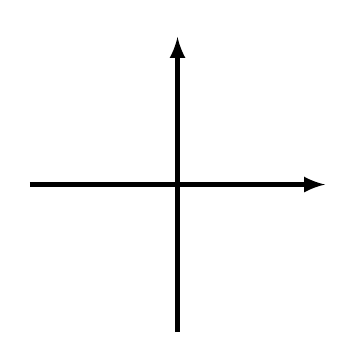
\begin{tikzpicture}[scale=0.75]
      \draw[ultra thick,->,>=latex] (-2.5,0)--(2.5,0) node[below] {};
      \draw[ultra thick,->,>=latex] (0,-2.5)--(0,2.5) node[left] {};         
    \end{tikzpicture}
    \end{center} 
\fi
\fi




\ifnum \Version=9
\question[3] Consider the system $$\vec x \, ' = A\vec x, \quad A = \begin{pmatrix} 1&-4\\1&3 \end{pmatrix}, \quad \vec x = \begin{pmatrix} x(t)\\y(t)\end{pmatrix} $$ The eigenvalues of $A$ are $\lambda = 2\pm i\sqrt 3$. Sketch the phase portrait of the system. Sketch at least two solution curves. Please indicate the direction of motion on your solution curves. Don't forget to label your axes.   

\ifnum \Solutions=1 {\color{DarkBlue} 
\textbf{Solutions:} solution curves should spiral away from the origin and rotate counter clockwise. Axes should be labelled. Ok to only draw only two solution curves. 
    \begin{center}
    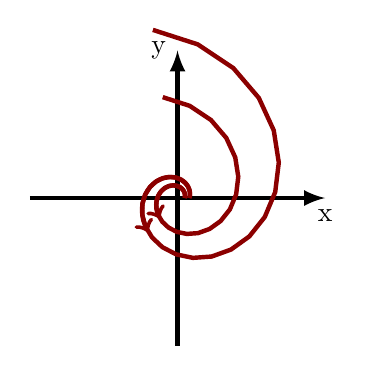
\begin{tikzpicture}[scale=0.75]
      \draw[ultra thick,->,>=latex] (-2.5,0)--(2.5,0) node[below] {x};
      \draw[ultra thick,->,>=latex] (0,-2.5)--(0,2.5) node[left] {y};      
      \draw[domain=0:8,ultra thick,samples=30,DarkRed] plot ({cos(deg(\x))*0.12*exp(\x/3)},{sin(deg(\x))*0.12*exp(\x/3)});
      \draw[domain=0:4,->,ultra thick,samples=30,DarkRed] plot ({cos(deg(\x))*0.12*exp(\x/3)},{sin(deg(\x))*0.12*exp(\x/3)});
      \draw[domain=0:8,ultra thick,samples=30,DarkRed] plot ({cos(deg(\x))*0.2*exp(\x/3)},{sin(deg(\x))*0.2*exp(\x/3)});
      \draw[domain=0:4,->,ultra thick,samples=30,DarkRed] plot ({cos(deg(\x))*0.2*exp(\x/3)},{sin(deg(\x))*0.2*exp(\x/3)});      
    \end{tikzpicture}
    \end{center} 
} 
\else 
    \begin{center}
    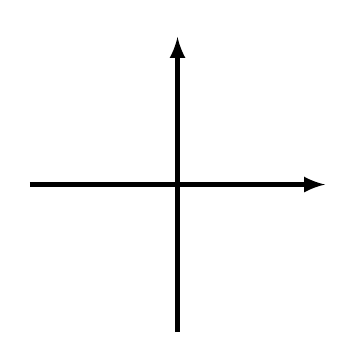
\begin{tikzpicture}[scale=0.75]
      \draw[ultra thick,->,>=latex] (-2.5,0)--(2.5,0) node[below] {};
      \draw[ultra thick,->,>=latex] (0,-2.5)--(0,2.5) node[left] {};         
    \end{tikzpicture}
    \end{center} 
\fi
\fi


